%\documentclass[11pt, a4paper, utf8x]{article}
%\documentclass[11pt, a4paper]{article}
\documentclass{iacas}
%
%\usepackage[utf8x]{inputenc}
\usepackage{amsmath}
\usepackage{amsfonts}
\usepackage{amssymb}
\usepackage{times}
\usepackage{color}
\usepackage{amsthm}
\usepackage{graphicx}
\usepackage{latexsym}
\usepackage{subcaption}
\usepackage{commath}
\usepackage{tikz}
\usepackage{hyperref}% embedding hyperlinks [must be loaded after dropping]
\usepackage{cleveref}
\usepackage{enumitem}
\usepackage{algorithm}
\usepackage[noend]{algpseudocode}
%\usepackage[english,hebrew]{babel}
%\usepackage{hebfont}
\captionsetup{compatibility=false}

%\usepackage[margin=2cm]{geometry}

%--Tikz defenitions--%
\usetikzlibrary{positioning}
\tikzset{main node/.style={circle,draw,minimum size=0.5cm,inner sep=0pt}}

\usepackage{amsmath}
%\usepackage{soul,color}
\usepackage{threeparttable}% tables with footnotes
\usepackage{dcolumn}% decimal-aligned tabular math columns

%--COMMANDS--%
\newcommand{\rsqr}{\mathbb{R}^2}
\newcommand{\rthrd}{\mathbb{R}^3}
\newcommand{\eqsn}[1]{\begin{equation}#1\end{equation}}
\newcommand{\br}{$\\ $}

\newcommand{\bmat}[1]{\begin{bmatrix}#1\end{bmatrix}}
\newcommand{\mat}[1]{\begin{matrix}#1\end{matrix}}
\newcommand{\vmat}[1]{\begin{vmatrix}#1\end{vmatrix}}

\newcommand{\con}{c\left(t\right)}
\newcommand{\conp}[1]{c_{#1}\left(t\right)}
\newcommand{\concov}{\mathtt{C}\left(\con\right)}
\newcommand{\concovp}[1]{\mathtt{C}\left(\conp{#1}\right)}
\newcommand{\conset}{\mathtt{G}}

\DeclareRobustCommand{\rchi}{{\mathpalette\irchi\relax}}
\newcommand{\irchi}[2]{\raisebox{\depth}{$#1\chi$}} % inner command, used by \rchi

\newtheorem{theorem}{Theorem}
\newtheorem{lemma}{Lemma}
\newtheorem{assumption}{Assumption}
\newtheorem{remark}{Remark}
\newtheorem{proposition}{Proposition}
\newtheorem{corollary}{Corollary}
\newtheorem{example}{Example}
\newtheorem{definition}{Definition}
\newtheorem{problem}{Problem}


\begin{document}
%--TITLE--%
\newcolumntype{d}{D{.}{.}{-1}}

\title{A Projected Lloyd's Algorithm for Coverage Control Problems}

\author{%
  Yoav Palti\thanks{Faculty of Aerospace Engineering, Technion - Israel Institute of Technology, Haifa, yoavp10@gmail.com}
  \ and
  Daniel Zelazo\thanks{Associate Professor, Faculty of Aerospace Engineering, Technion - Israel Institute of Technology, Haifa, dzelazo@technion.ac.il}
}

\maketitle

\begin{abstract}
This work presents a new approach for a coverage problem for large areas and a limited number of sensors. We consider the problem where there are not enough sensors to provide complete coverage of the designated area at once, and therefore the sensors should coordinate their coverage in a sequential manner.  Furthermore, we require that at each stage of coverage, a sub-region in the area is constantly monitored. Our solution approach is a combination of two algorithms, the first one is Lloyd's algorithm, which is well known and used in this field, and the second one is a modified Lloyd's algorithm that we term the \emph{projected Lloyd's Algorithm}. We demonstrate our results with numerical simulations.
%\textcolor{red}{One paragraph abstract summarizing work required here}
\end{abstract}

\section{Introduction}
The mission of monitoring some area using sensors is widely spread in various fields - it can be used for photographing a large area, receiving or sending electromagnetic signals, tracking targets, or even for designing an algorithm for a robotic vacuum cleaner \cite{Nigam2012, 7798796, 7798244}.
%
This research area is known in the scientific community as the \emph{coverage control} problem \cite{Cassandras2005}. Sensor coverage can be generally described as the reflection of how well a given range (for example, area) is monitored by sensors. This field is well explored in the scientific community, especially in the recent years when the fields of distributed algorithms and cooperative systems were developed.

When coverage is required for large areas, and specifically when a single sensor cannot provide full coverage of that area, the idea of using a \emph{formation} of mobile sensors is presented \cite{Hokayem2007}. The main advantage of using a formation is the ability to perform a task in a distributed way, which leads to cheaper sensors, objective flexibility, and survivability (the system can function even if one of the sensors is broken) \cite{Cortes2004}.

A concept that repeats in many researches is finding a set of trajectories (at least one route for every sensor), allowing the mobile sensors to achieve the required coverage goal.  For example, when trying to cover an area using two mobile sensors, the algorithm will define a trajectory for each sensor such that the whole area will be covered \cite{Atinc2013,Hussein2007}.
Another idea that appears in most of the relevant literature is the use of Voronoi diagrams for optimizing the sensor location \cite{Cortes2004,Hussein2007}. 

To the best of out knowledge, there isn't any solution that tries to deal with the coverage problem in the scenario where, on the one hand, an operator has to maintain coverage of a specific part of the area, and on the other hand, have a set of formations that all together provides a complete coverage of the area. In this research, we developed a new coverage algorithm that deals with this problem. The operator can switch formations on different parts of the area and get a static coverage on some part of the whole area. For this algorithm, we defined a coverage constraint, that defines an area that at least one agent has to be present in at all steady-state times. This constraint represent, for example, an agent that must be within the home-station coverage radius. 

%\textcolor{red}{(summary of the work/contribution should be more clearly motivated, stated, and explained in intro)}

%\textcolor{red}{(include brief outline (in text) of the paper layout)}
Following this chapter, this extended abstract will include a brief background about Voronoi Diagrams and general coverage algorithms. After it, the problem will be formally formulated, and later a solution will be introduced.

\section{Voronoi Diagrams and Distributed Coverage Algorithms}
%\textcolor{red}{(provide short paragraph summarizing what you will talk about here)}
In this chapter we will introduce two main concepts that were used in this work. First, Voronoi Diagrams, and later Lloyd's algorithm.
\subsection{Voronoi Diagrams}
The basic mathematical concept that we employ in this work is the \emph{Voronoi Diagram}. While being a method to partition an area with some cost function, the is a widely-used representation in the coverage problem \cite{Cortes2004,Hussein2007, Du1999}. The Voronoi Diagram of a region $\Omega \subset \rsqr$ is the set of partitions $\mathcal{V} = \left\{V_{i} \mid \cup V_{i} = \Omega\right\}$, generated by the generators $\mathcal{Z} = \{z_1,\ldots,z_n\mid z_{i} \in \Omega\}$, such that
\begin{equation} \label{Voronoi Definition}
V_{i} = \{q\in\Omega \mid \norm{q - z_i} \leq \norm{q - z_j} \forall z_i,z_j\in\mathcal{Z}\},
\end{equation}
where $V_{i}$ corresponds to the $i$-th element of $\mathcal{Z}$, and $\norm{\cdot}$ denotes the Euclidean distance.

A more intuitive and non-formal definition of the Voronoi Diagram is as follows. If we take some area and place points $p_i$ in it, then each partition is the set of all points that are closer to $p_i$ than $p_j$, when $j \neq i$. An example is the problem where we have post offices in some city, and we need to decide which house will be served by which post office branch. Using Voronoi partitioning, we can determine which houses are the nearest to each branch and therefore conclude which houses each branch will serve.
%\textcolor{red}{(now explain in basic words what a voronoi partition is!)}

One can define a density function, $\rho_i$, for each Voronoi partition $V_{i}$. Then, we can define the center of mass for each partition as
\begin{equation}
z_{i}^{*} = \frac{\int_{V_{i}}y\rho(y)dy}{\int_{V_{i}}\rho(y)dy}.
\end{equation}
If a generator $z_{i} = z_{i}^{*} \, \forall \,V_{i}$, we call this partitioning a \emph{centroidal Voronoi tessellation} (CVT). Such tessellations are useful in terms of location optimization \cite{Cortes2004,Du1999,Atinc2013}.
A Voronoi tessellation illustration can be seen in Figure~\ref{fig:Voronoi_tessellation_illustration}. Going back to the post-office example, the CVT can help us determine where those post office branches should be located for an optimal distribution of houses per branch.

\begin{figure}[!ht]
\centering
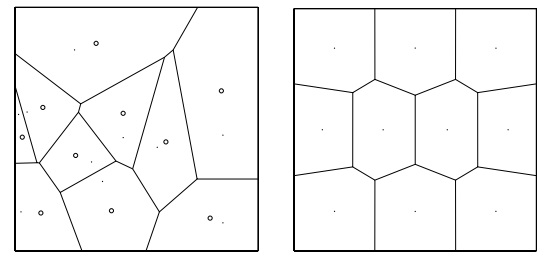
\includegraphics[scale=0.5]{figures/voronoi_partitioning.jpg}
\caption{An illustration of Voronoi diagrams. On the left, a regular Voronoi diagram, and on the right, a centroidal Voronoi tessellation. The figure is taken from \cite{Du1999}.} %\textcolor{red}{(for final submission, generate your own example/figures)}}
\label{fig:Voronoi_tessellation_illustration}
\end{figure}

As can be seen in equation (\ref{Voronoi Definition}), the calculation of each Voronoi cell for some agent depends on the other agents positions. Therefore, any sort of calculation required \emph{sharing information}. This can be done in a centralized approach (as it was done for this research), but there exists also decentralized calculations, for example \cite{Adams2009}. Using decentralized calculation, each agent have to have the info only on their neighbours (or any limited amount of agents), which allows for calculating huge networks, in dynamic situations where agents can, for example, connect and disconnect from the network in real time.

\subsection{Lloyd's Algorithm}
As mentioned above, the CVT's are very useful for locational optimization. However, calculating the CVT might be a complicated task. Lloyd proposed a very simple way of calculating the CVT \cite{Lloyd1982}, presented in Alogirthm \ref{LloydAlgo}. %\textcolor{red}{(please use a latex algorithm environment for describing algorithms)}
\begin{algorithm}
\caption{Lloyd's Algorithm}\label{LloydAlgo}
\begin{algorithmic}[1]
\State Calculate the Voronoi diagram for the current agents positions.
\State Calculate the center of mass for every cell.
\State Move the agents to the center of mass.
\end{algorithmic}
\end{algorithm}

%\begin{enumerate}
%\item Calculate the Voronoi diagram for the current agents positions.
%\item Calculate the center of mass for every cell
%\item move the agents the center of mass
%\item repeat until converge
%\end{enumerate}
Cortes et al. proposed a control algorithm based on Lloyd's algorithm \cite{Cortes2004}. According to \cite{Cortes2004}, if we define agent $i$ position as $p_i$ and the $i$'s partition centroid as $C_{V_{i}}$, then for some proportional constant $k_{prop}$, the controller can be defined as:
\begin{equation} \label{LloydsContol}
u_{i} = -k_{prop}\left( p_i - C_{V_{i}} \right)
\end{equation} 
%
Another thing to notice is that one can modify the density function, which will change the geometrical position of the centroid.

%\textcolor{red}{(what is missing in this section is the idea that this is a cooperative/distributed calculation, and neighbors share information - this is important!)}

\section{Problem Formulation}
Let us consider an area $A \subset \rsqr$ that we aim to cover with $n \in \mathbb{N}$ \emph{mobile} sensors. Those sensors are defined as the set $S = \{s_1, \ldots, s_n\}$ located at positions $P(t) = \{ p_i (t) \in \rsqr \mid i = 1,\; \ldots ,\; n\}$:
\begin{itemize}
\item The mobile sensors are modelled using integrator dynamics $\dot{p_i}(t)=u$.
\item Each sensor can cover an area described by the abstract set $C_i \left( p_i(t) \right) \subset \rsqr$.
\end{itemize}

\subsection{Configuration}
A configuration $c$ of the mobile sensors at time $t$ is the stack of the sensor positions at time $t$:
\begin{equation*}
c\left(t\right) = \bmat{
p_{1}^{T}\left(t\right)&\cdots&p_{n}^{T}\left(t\right)}^{T}\in\mathbb{R}^{2n}
\end{equation*}
Thus the coverage of a configuration:
\begin{equation*}
D\left( c\left( t \right) \right) = \cap C_i(p_i(t))
\end{equation*}
Let us consider a sub-area of $A,\; A_m \subset A$ which must be partially covered (e.g. ground station).

\begin{assumption}
$D\left( c\left( t \right) \right) \subset A$ - a single configuration \emph{can't} provide full coverage!
\end{assumption}

\subsection{Partition}
The partition of $A \in \rsqr$, $PR(A)$, is a finite set built from $n$ subset $pr_i \subset \rsqr,\; i=1,\; \ldots,\; n$ such that:
\begin{itemize}
\item $pr_i \cap pr_j = \emptyset \; \forall i \neq j$.
\item $\cup pr_i = A$.
\end{itemize}

\begin{figure}[!ht]
\centering
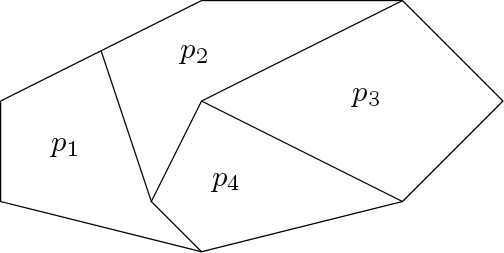
\includegraphics[scale=0.6]{figures/problem-def/partitioning.png}
\caption{An example of a partition of some area $PR(A)$}
\end{figure}

\subsection{Problem Definition}
\begin{problem} \label{GeneralProblem}
\begin{enumerate}
\item Find a partition $PR(A)$ such that each subset $pr_i \in PR(A), \; pr_i \cap A_m \neq \emptyset$
\item Find a deployment controller, such that $$ pr_i \subseteq \lim_{t\rightarrow \infty}D(c(t)),\text{for }i=1,\ldots,n.$$
\end{enumerate}
\end{problem}

\section{Proposed Solution}
Assuming that there are no constraints at all, we propose an algorithm to solve the problem mentioned above:
\begin{algorithm}
\caption{Problem (\ref{GeneralProblem}) Solution Algorithm}\label{GeneralProbSolution}
\begin{algorithmic}[1]
\State Using some random initial guess, calculate the CVT for the whole area.
\State For each partition (assuming that the agents can actually cover each partition with their coverage radius), calculate the CVT. The initial positions for the CVT calculation is the previous partition CVT.
\end{algorithmic}
\end{algorithm}
%\begin{enumerate}
%\item Using some random initial guess, calculate the CVT for the whole area
%\item for each partition (assuming that the agents can actually cover each partition with their coverage radius), calculate the CVT. The initial positions for the CVT calculation is the previous partition CVT
%\end{enumerate}

We should notice the following things:
\begin{enumerate}
\item In stage 1, the number of the partition that the area will be divided to is somewhat arbitrary.
\item In stage 2, we assume that the coverage radius of the agents is big enough to cover the whole partition. If it's not the case, then we can dived the area for more partitions in stage 1. Some more advanced work can propose an algorithmic solution for this problem.
\item The Voronoi diagram can be calculated even if the agents are outside of the required area. It does require sometimes more iterations.
\end{enumerate}

However, as one can see, we didn't answer the area constraint.
\subsection{Projected Lloyd's Algorithm}
An approach to ensure the area constraint is to modify the original Lloyd's algorithm. If we use the \emph{Projection Operator} on the cell's center of mass, then the control law \ref{LloydsContol} will be now:
\begin{equation} \label{ProjectedLloydsContol}
u_{i} = -k_{prop}\left( p_i - \textit{proj}\left( C_{V_{i}} \right) \right)
\end{equation} 

Formulating this as an algorithm:
\begin{algorithm}
\caption{Projected Lloyd's Algorithm}\label{ProjLloydsAlgorithm}
\begin{algorithmic}[1]
\State Calculate the Voronoi diagram for the current agents positions.
\State Calculate the center of mass for every cell.
\State Project the center of mass of every cell to the area constraint limiting polygon.
\State Move the agents the projected center of mass.
\State Repeat until converge.
\end{algorithmic}
\end{algorithm}

%\begin{enumerate}
%\item Calculate the Voronoi diagram for the current agents positions.
%\item Calculate the center of mass for every cell
%\item Project the center of mass of every cell to the area constraint limiting polygon
%\item move the agents the projected center of mass
%\item repeat until converge
%\end{enumerate}

As one can see, we added two more steps over the original Lloyd's algorithm - where we project the cell center of mass to the polygon that defines the area constraint (steps number 3-4), and then moving the agents to those points. Those step allows us to ensure that at least one agent will be \emph{on} the limiting polygon, thus we will have coverage within the constraint.

\subsubsection{Stability of the Projected Lloyd's Algorithm}
\begin{theorem}
The controller proposed in (\ref{ProjectedLloydsContol}) is locally asymptotical stable.
\end{theorem}

Full proof will be given in the final version. However, in \cite{Cortes2004}, we can find a proof for the stability of Lloyd's algorithm in the form of controller. We added one linear step to this solution, and it is very easy to see that this does not affect the Lyaponov function.

%\textcolor{red}{(you should provide a formal Theorem statement and say proof will be given in final version)}

\subsection{Results}
First of all, we shall show the difference between the constrained and non constrained CVT:
\begin{figure}[!ht]
\centering
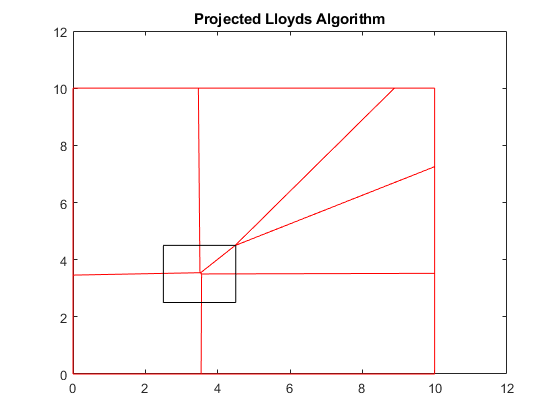
\includegraphics[scale=0.5]{figures/results/constrainedVoronoi.png} 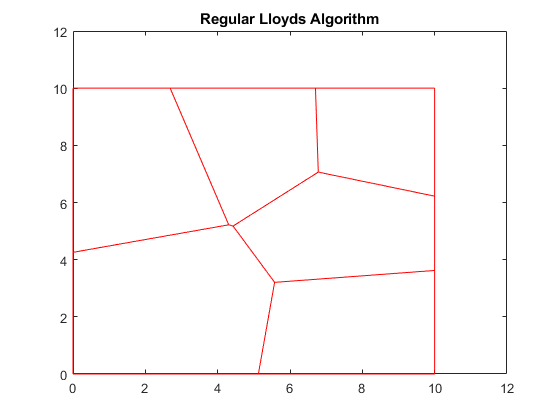
\includegraphics[scale=0.5]{figures/results/unconstrainedVoronoi.png}
\caption{Projected vs. Regular Lloyd's algorithm}
\end{figure}

Next thing is to see the different agents formations within each area partition. The following example is for the projected case, and the order of the partitions that are being covered is arbitrary (i.e. in step $i+1$ the partition covered is not necessarily adjacent to the once that was covered in step $i$):
First of all, we shall show the difference between the constrained and non constrained CVT:
\begin{figure}[!ht]
\centering
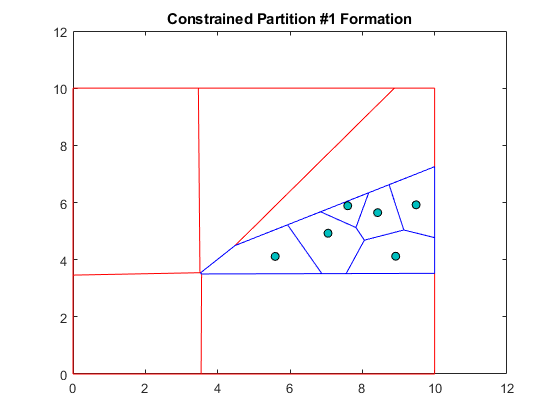
\includegraphics[scale=0.3]{figures/results/constrainedStep1.png} 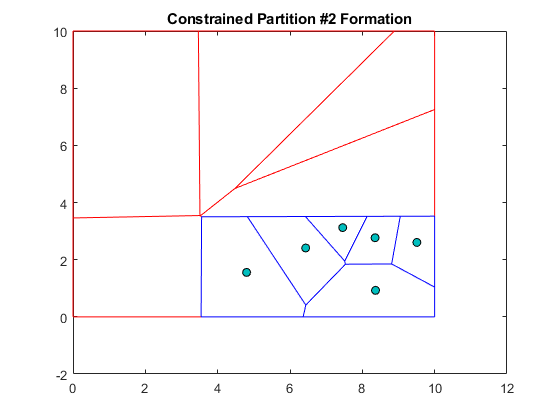
\includegraphics[scale=0.3]{figures/results/constrainedStep2.png} 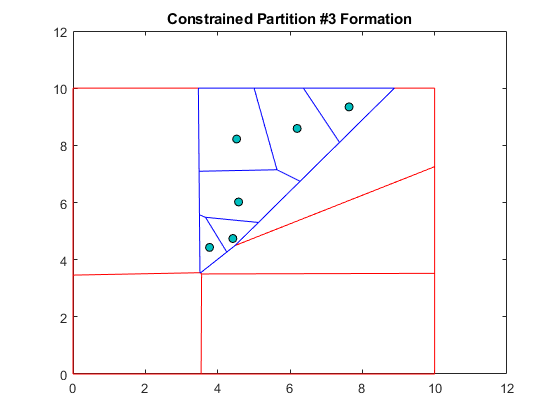
\includegraphics[scale=0.3]{figures/results/constrainedStep3.png} 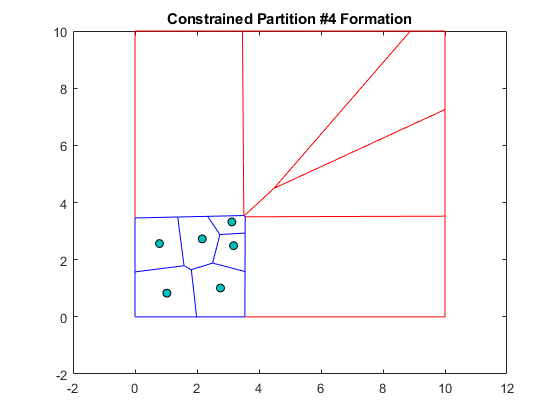
\includegraphics[scale=0.3]{figures/results/constrainedStep4.png} 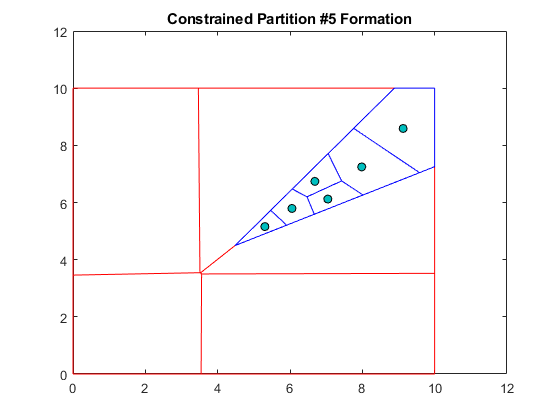
\includegraphics[scale=0.3]{figures/results/constrainedStep5.png} 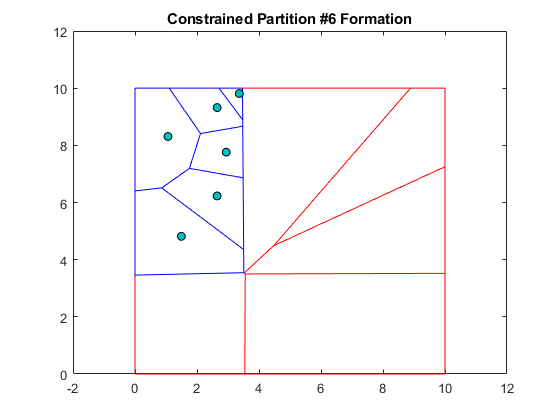
\includegraphics[scale=0.3]{figures/results/constrainedStep6.png} 
\caption{Covering different partitions in an arbitrary order}
\end{figure}

\section{Concluding Remarks}
The Coverage Problem is well known and researched. This work provides a new approach for the common problem of not having enough sensors, and deals with it from a static point of view, while maintaining coverage on some constrained area.\\
The proposed solution is a simple control law which, under the work assumption, solves the problem. The simplicity of the control law, all together with the fact its stability, open the way for combining it with other control laws in some future work, which might lead to some interesting results. For example, combining this controller with a formation control controller, together with calculating the Voronoi in a distributed way, can lead to some interesting results for autonomous, dynamically changed swarms.
%\textcolor{red}{add concluding statements - including idea of using formation control in work)}
\bibliography{bibliography}
\bibliographystyle{iacas}
\end{document}
